% !TeX program = xelatex
% !TeX encoding = UTF-8
\documentclass[UTF8]{standalone}
\usepackage{tikz,newtxmath,esint,ctex}
\usepackage{fontspec}
\usepackage{libertine}
\usepackage{pgf} % for the calculation
% \libcirc and \libcircblk display their '0' if the parameter is out of range
\newcommand{\libcirc}[1]{\pgfmathparse{
    ifthenelse(#1 > 0 && #1 < 21, Hex(9311+#1), Hex(9450)
    }\libertineGlyph{uni\pgfmathresult}}
\newcommand{\libcircdbl}[1]{\pgfmathparse{Hex(9460+#1)}\libertineGlyph{uni\pgfmathresult}}
\newcommand{\libcircblk}[1]{\pgfmathparse{
    ifthenelse(#1 > 0 && #1 < 11, Hex(10101+#1),
        ifthenelse(#1 > 10 && #1 < 21, Hex(9450-10+#1),
            Hex(9471)
        )
    )
    }\libertineGlyph{uni\pgfmathresult}}

\newcommand{\juncirc}[1]{{\fontspec[Ligatures=Discretionary]{Junicode}[#1]}}
\newcommand{\juncircdbl}[1]{{\fontspec[Ligatures=Discretionary]{Junicode}[[#1]]}}
\newcommand{\juncircblk}[1]{{\fontspec[Ligatures=Discretionary]{Junicode}<#1>}}

\usepackage{pgffor} % just for the demo loop
\setlength{\parindent}{0pt} % just for the demo
\begin{document}
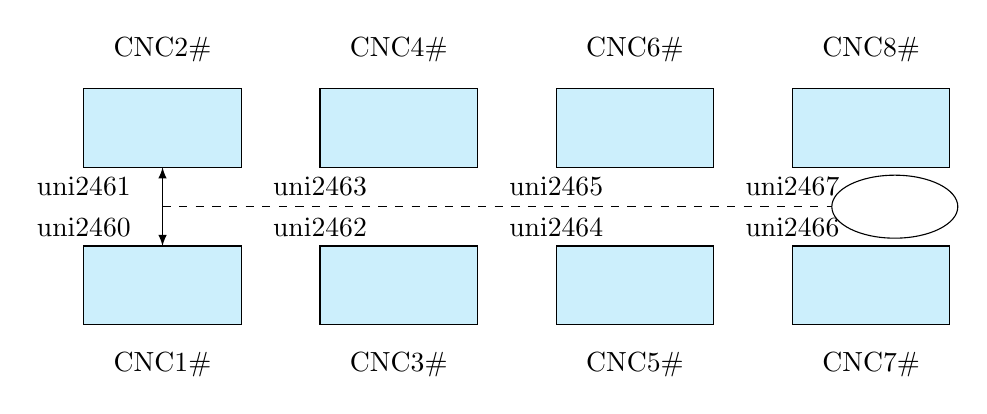
\begin{tikzpicture}
    \filldraw[fill=cyan!20] (0,0) rectangle (2,1);
    \filldraw[fill=cyan!20] (3,0) rectangle (5,1);
    \filldraw[fill=cyan!20] (6,0) rectangle (8,1);
    \filldraw[fill=cyan!20] (9,0) rectangle (11,1);
    \filldraw[fill=cyan!20] (0,2) rectangle (2,3);
    \filldraw[fill=cyan!20] (3,2) rectangle (5,3);
    \filldraw[fill=cyan!20] (6,2) rectangle (8,3);
    \filldraw[fill=cyan!20] (9,2) rectangle (11,3);

    
    \draw[latex-latex] (1,1) -- ++ (0,1);
    
    \draw[dashed] (1,1.5) -- ++ (8.5,0);
    \draw (10.3,1.5) ellipse (0.8 and 0.4);
    \node at (1,-0.5) {CNC1\#};
    \node at (4,-0.5) {CNC3\#};
    \node at (7,-0.5) {CNC5\#};
    \node at (10,-0.5) {CNC7\#};
    \node at (1,3.5) {CNC2\#};
    \node at (4,3.5) {CNC4\#};
    \node at (7,3.5) {CNC6\#};
    \node at (10,3.5) {CNC8\#};

    \node[above] at (0,1) {\libcirc{1}};
    \node[above] at (3,1) {\libcirc{3}};
    \node[above] at (6,1) {\libcirc{5}};
    \node[above] at (9,1) {\libcirc{7}};
    \node[below] at (0,2) {\libcirc{2}};
    \node[below] at (3,2) {\libcirc{4}};
    \node[below] at (6,2) {\libcirc{6}};
    \node[below] at (9,2) {\libcirc{8}};
\end{tikzpicture}
\end{document}